\section{Simulation Study}\label{app:simstudy}

This section presents a simulation study evaluating the performance of our proposed estimators on a known data-generating process. The first subsection outlines our simulation study. The section section presents selected results about the bias and mean-square error of our estimators, and the coverage rates for our proposed variance estimation procedure.

\subsection{Study design}

We first generate data according to a known and evaluate the performance of different estimators. For all models we consider the data generating process:

\begin{align*}
Y_{sc} \sim N(X_{1, sc} + X_{2, sc} + X_{3, sc}, \sigma^2_{\epsilon} + \sigma^2_{\varepsilon})
\end{align*}

where $\sigma^2_{\varepsilon}$ represents the variance component from a state-level random effect, and $\sigma^2_{\epsilon}$ represents a variance component from a CPUMA-level random effect. Thus the errors in the model for $Y \mid X$ are equicorrelated within state with correlation $\rho$ equal to $\frac{\sigma^2_{\varepsilon}}{\sigma^2_{\epsilon} + \sigma^2_{\varepsilon}}$

We next define a correlation structure among our observed covariates. Specifically, we generate each covariate vector $X_{sc}$:

\begin{align*}
X_{sc} \sim N(\mu_s, \Sigma_{Q}) \\
\mu_j \sim N(0, \Sigma_{S}) \\
\end{align*}

Define $\Sigma_X = \Sigma_Q + \Sigma_S$. Let $\sigma^2_{x, j}$ be the j-th diagonal element of $\Sigma_X$ (and define $\sigma^2_{q, j}$ and $\sigma^2_{s, j}$ analogously). Across all simulations, we fix $\sigma^2_{x, j} = 2$. We also fix the off-diagonal elements of both $\Sigma_Q$ and $\Sigma_S$ to be equal and so that $Cor(X_j, X_k) = 0.25$. Finally, define $\rho_x = Cor(X_{sc}, X_{sd})$ for $c \ne d$; in other words, $\rho_x$ is the within-state correlation of the covariates $X_{sc}$, which we set to be equal for all covariates.

We also consider samples of size $m = 25$ states each with $p_s$ units and $n$ total units. We draw $p_s \stackrel{iid}\sim \lfloor Exp(0.1) + 10\rfloor$ so that the average number of regions per state is approximately 20 (and the approximate number of total units $n$ is on average approximately 450).

We next generate our noisy outcome and covariate estimates $(J, W)$:

\begin{align*}
(J_{sc}, W_{sc}) \stackrel{iid}\sim N((Y_{sc}, X_{sc}), \Sigma_{\nu, sc})
\end{align*}

\begin{align*}
    \Sigma_{\nu} = \begin{pmatrix}
    \sigma^2_{\nu, sc} & 0 & 0 & 0 \\
    0 & \sigma^2_{\nu, sc} & 0 & 0 \\
    0 & 0 & \sigma^2_{\nu, sc} & 0 \\
    0 & 0 & 0 & \sigma^2_{\nu, sc}
    \end{pmatrix}
\end{align*}

First, define $\rho_y = \sigma^2_{\varepsilon}/(\sigma^2_{\epsilon} + \sigma^2_{\varepsilon} + \sigma^2_{\nu})$. In other words, $\rho_y$ represents the within-state correlation of the outcome model errors, including the measurement errors in the outcome. We fix this to be 0.25 throughout all simulations.

We allow $\sigma^2_{\nu, sc}$ to be a function of the sample size of an underlying survey that generates the estimate. We simulate these sample sizes $r_{sc}$ drawn from some distribution (see more on this below). Let $R_{sc}$ be a 3x3 diagonal matrix with diagonal elements $r_{sc}$. Let $\sigma_{\nu}^{2\star}$ be defined as the limit as $n \to \infty$ of $n^{-1}\sum_{sc}\sigma^2_{\nu, sc}$ (we ensure this limit exists). Let $\tau = \sigma^2_x/\sigma^2_w$. We then fix a value $\sigma_{\nu}^{2\star}$ so that that as $n \to \infty$, $n^{-1} \tau \sum_{sc}\frac{\sigma^2_{\nu}}{r_{sc}} \to^p \sigma^2_{\nu}$. In other words, $\sigma_{\nu}^2$ represents the common variance that generate all errors in the ``heterogeneous adjustment'' model. We also simulate homoskedastic measurement errors, letting $\sigma^2_{\nu, sc} = \sigma^2_{\nu}$. 

For our simulations we generate population datasets of $m = 5000$ that consider all XX combinations of the following parameters:

\begin{itemize}
    \item $(r_{sc} \sim Unif(300, 2300), r_{sc} = 1)$ 
    \item $\rho_x \in \{0, 0.25, 0.5\}$
    \item $\tau \in \{0.95, 0.9, 0.85\}$
\end{itemize}

For each parameterization we take 500 random samples of size $m = 25$ and estimate H-SBW weights with targeting $\upsilon_0 = c(1, 1, 1)$. We set $\delta = 0$ and consider $\rho \in \{0, 0.25, 0.5\}$. We then estimate weights that reweight the following datasets to $\upsilon_0$: ($W_{A=1}$, $X_{A=1}$, $\tilde{X}_{A=1}^{hom}$, $\tilde{X}_{A=1}^{hom}$, $\tilde{X}_{A=1}^{cor}$), as defined in Appendix~\ref{app:adjustmentdetails}. We estimate the variance for each estimator using the leave-one-state-out jackknife, described in Section~\ref{sec:methods}.
 
Note: for $\hat{\kappa}$ we use the empirical covariance matrix of $W$, the estimated means $\bar{W}$, and $\hat{\Sigma}_{\nu, sc}$, where we draw $\hat{\Sigma}_{\nu, sc}$ from $\Sigma_{\nu, sc} + N(0, 0.001*n*I_d)$. In other words, when averaged together we assume that $\hat{\Sigma}_{\nu}$ have a fairly precise estimate of $\Sigma_{\nu}$.

\subsection{Selected results}

We present selected results from this study. We consider where the measurement error variances are heterogeneous (i.e. the ``heterogeneous adjustment'' model is correct). Figure~\ref{fig:simbias} displays the bias associated with each estimator. From left to right, the panels reflect different values of $\tau = \sigma^2_x/\sigma^2_w$ -- the left-most panels have the most measurement error while the right-most panels have the least. From top to bottom the panels reflect different values of $\rho_x$: the top-most panel has no correlation structure among the covariates, while the bottom-most panels are more highly correlated within state. Within each panel we organize each result by which covariate set was balanced: $W$ represents the estimators generated without any covariate adjustment; $X$ reflects estimators generated on the true covariates; ``Xhat-het'' ($\hat{X}_{A=1}^{het}$) represents the heterogeneous adjustment, ``Xhat-hom'' ($\hat{X}_{A=1}^{hom}$) represents the homogeneous adjustment, and ``Xhat-cor'' ($\hat{X}_{A=1}^{cor}$) represents the correlated adjustment. The estimators are colored by the assumed value of $\rho$ in the H-SBW objective: across all simulations, the true correlation for the outcome model ($\rho_y$) is again 0.25.

We highlight a few interesting results. First, if we know the true values of $X$, we see that all of our estimators are unbiased estimate. However, we see that balancing on $W$ results in bias, and the bias increases as $\tau$ decreases. Third, setting $\rho > 0$ exacerbates this bias: this aligns with our expectations from Remark~\ref{rmk:glsbias}, when we considered GLS weights in the context of measurement error.

We then try to mitigate this bias by using some estimate of $\mathbb{E}[X \mid W, A]$. We see that when the covariates  uncorrelated (i.e. the top set of panels), balancing on $X$, $\hat{X}_{A=1}^{hom}$, $\hat{X}_{A=1}^{het}$, or $\hat{X}_{A=1}^{cor}$ results in approximately unbiased estimates for all values of $\rho$. This aligns with our theoretic results in Appendix~\ref{app:AsecI}. However, we also see that when $X$ are correlated, setting $\rho > 0$ results in biased estimates for $\hat{X}_{A=1}^{het}$ or $\hat{X}_{A=1}^{hom}$; however, we still obtain approximately unbaised estimates for $\rho = 0$ (SBW). Even so the bias from H-SBW is still much less than the bias for the corresponding estimates that balance on $W$ when using $\hat{X}_{A=1}^{het}$ or $\hat{X}_{A=1}^{hom}$.

Interestingly, our proposed adjustment to asymptotically remove the bias from H-SBW -- $\hat{X}_{A=1}^{cor}$ -- appears to make this bias worse given the sample size considered here. In Section~\ref{appssec:simstudyresults2}, we show results verifying that this procedure is consistent as we increase $m$.

\begin{figure}[H]
\begin{center}
    \caption{Simulation study: estimator bias}\label{fig:simbias}
    \label{fig:loveplotc1}
    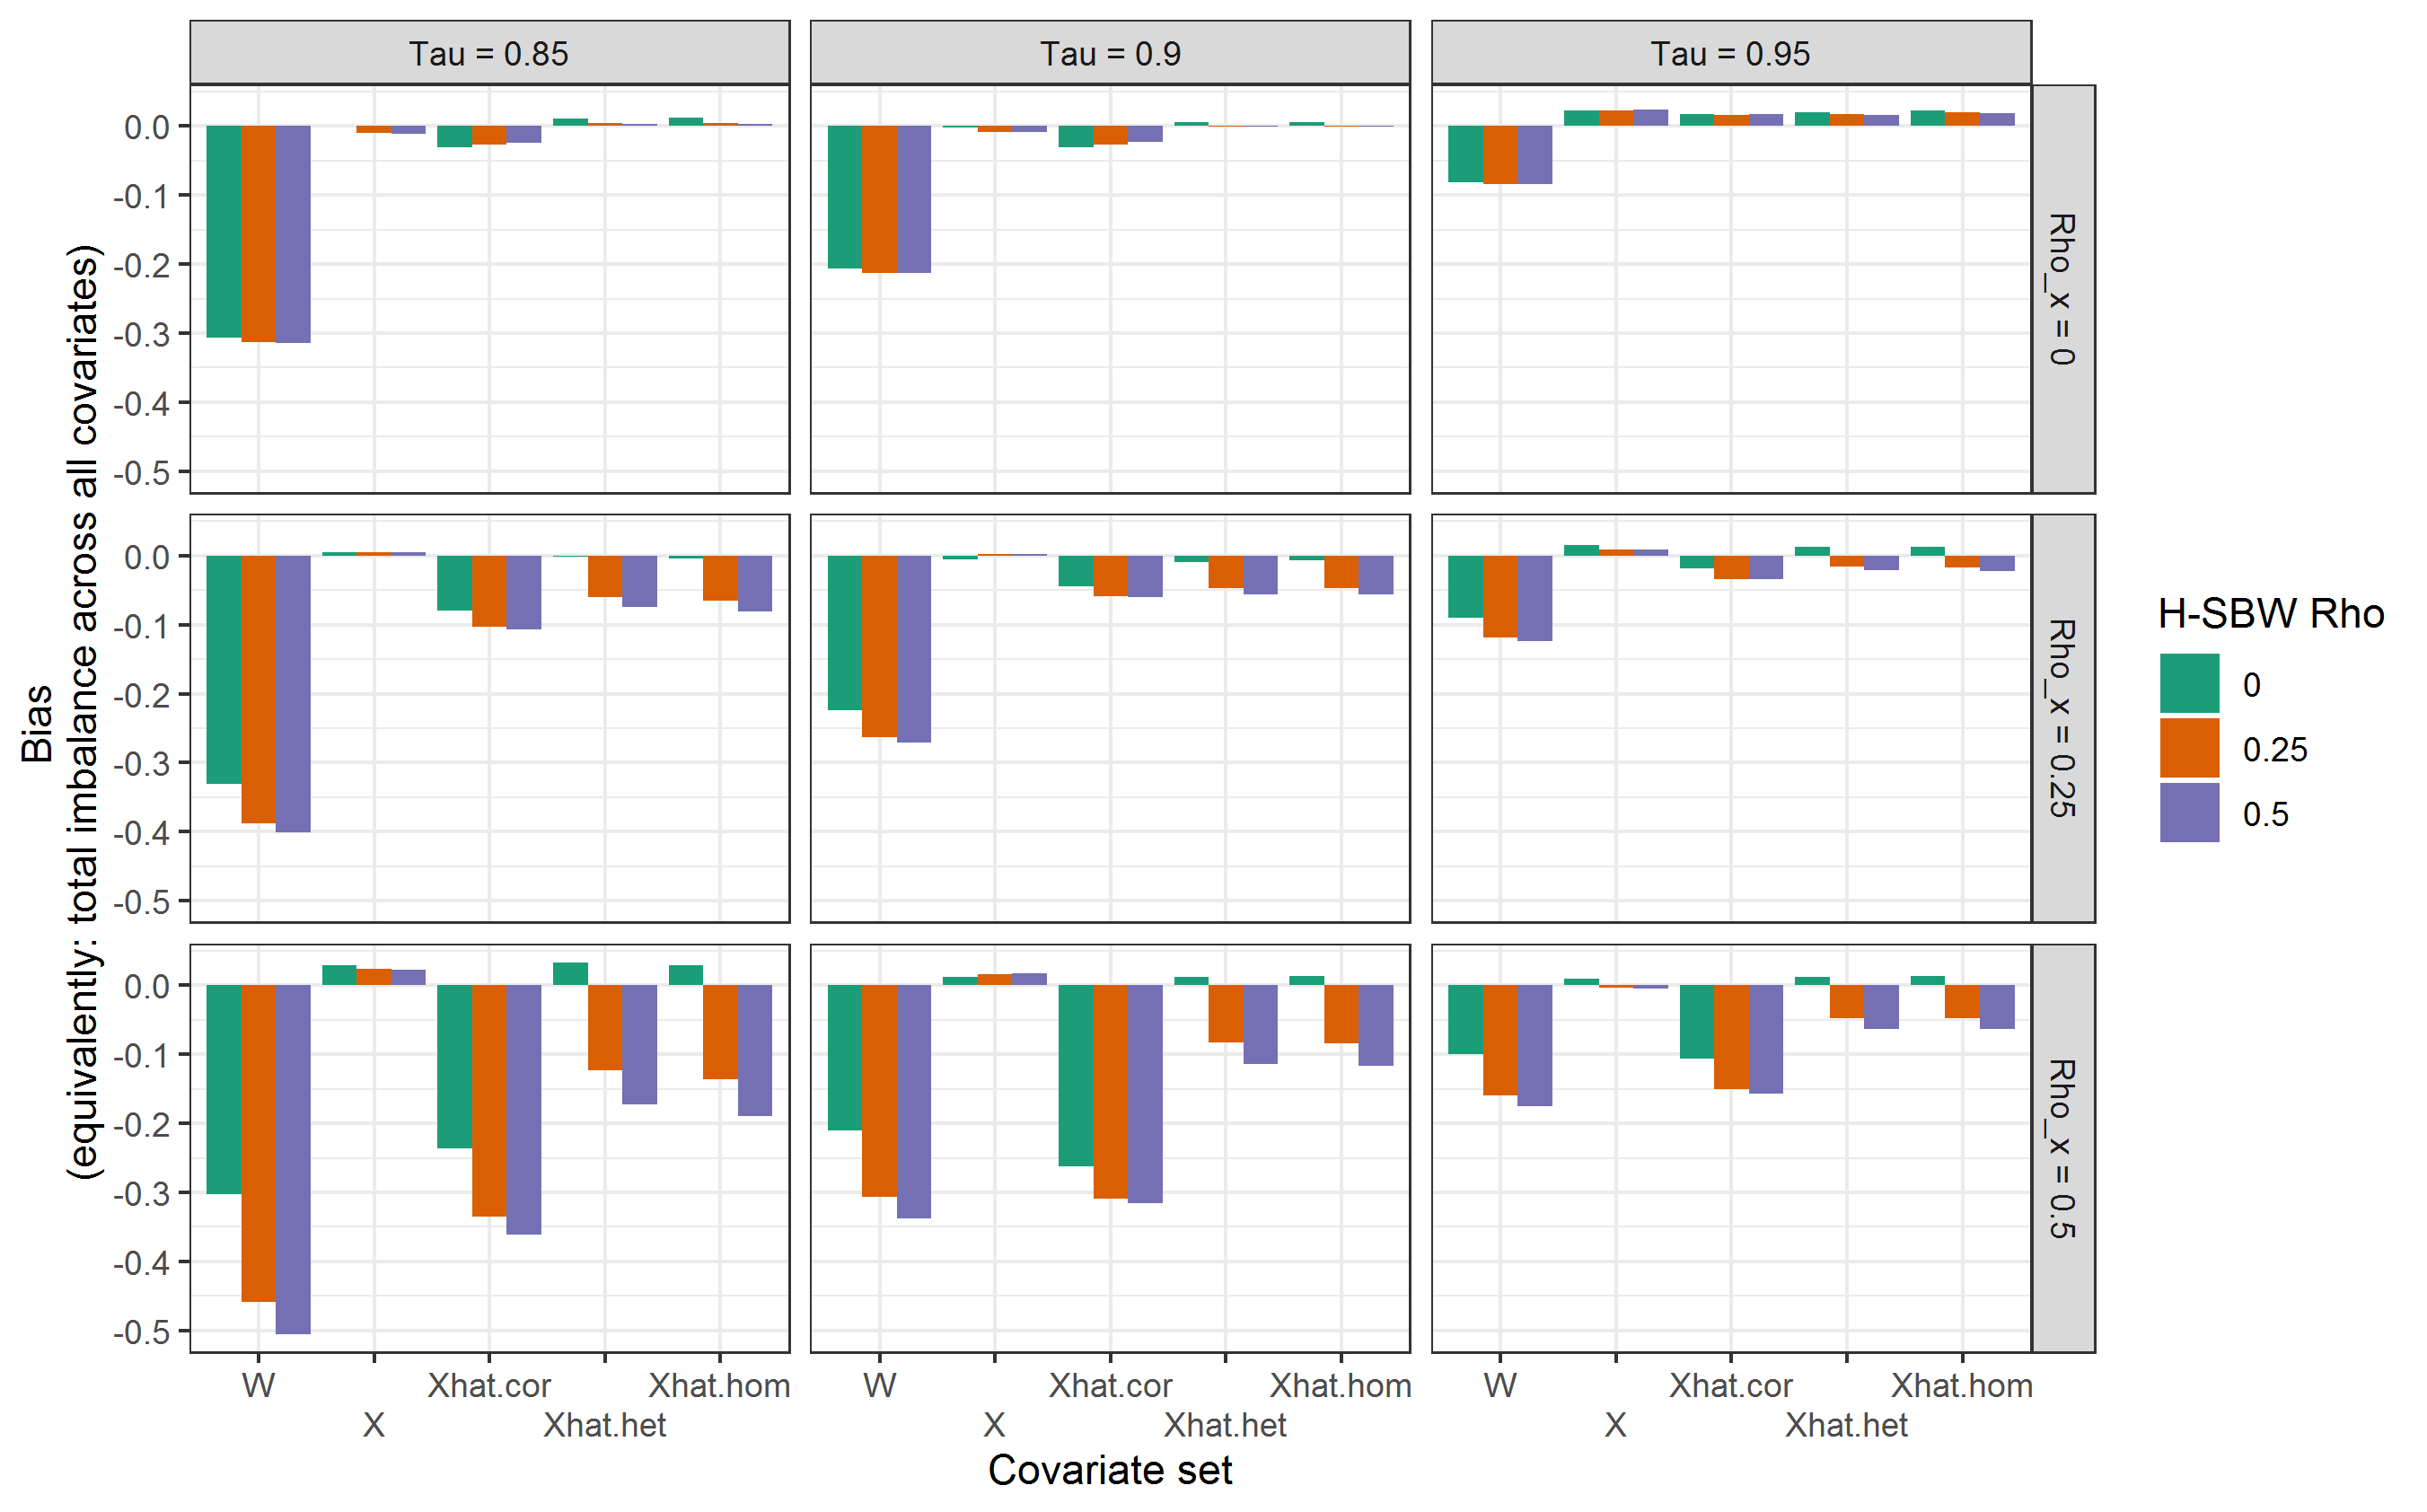
\includegraphics[scale=0.5]{01_Plots/bias-plot.png}
    \subcaption{Averaged across 500 simulations for each specification}
\end{center}
\end{figure}

All of these simulations had heterogeneous measurement. When we examine the results when the errors are homogeneous (results not displayed but available on request), we find that the estimators that balance on $\tilde{X}^{het}_{A=1}$ have a small bias even when $\tau = 0$ or $\rho = 0$. Assuming this model is correct when it is not appears to have some cost. This may help explain the worse performance we found when applying the heterogeneous adjustment to our validation study in Section~\ref{sec:results}.

We next calculate the variance our estimates across all simulations and display these results in Figure~\ref{fig:simvar}. Unsurprisingly, we find that we obtain a modest variance reduction as we increase $\rho$. Interestingly, even when $\rho$ is incorrect (assumed $0.5$ instead of $0.25$), we tend to get nearly identical improvements to $\rho = 0.25$. We also see that balancing on $\tilde{X}^{cor}_{A=1}$ can lead to a much more variable estimate, again suggesting a large cost to using this procedure given a small sample size.

\begin{figure}[H]
\begin{center}
    \caption{Simulation study: estimator variance}\label{fig:simvar}
    \label{fig:loveplotc1}
    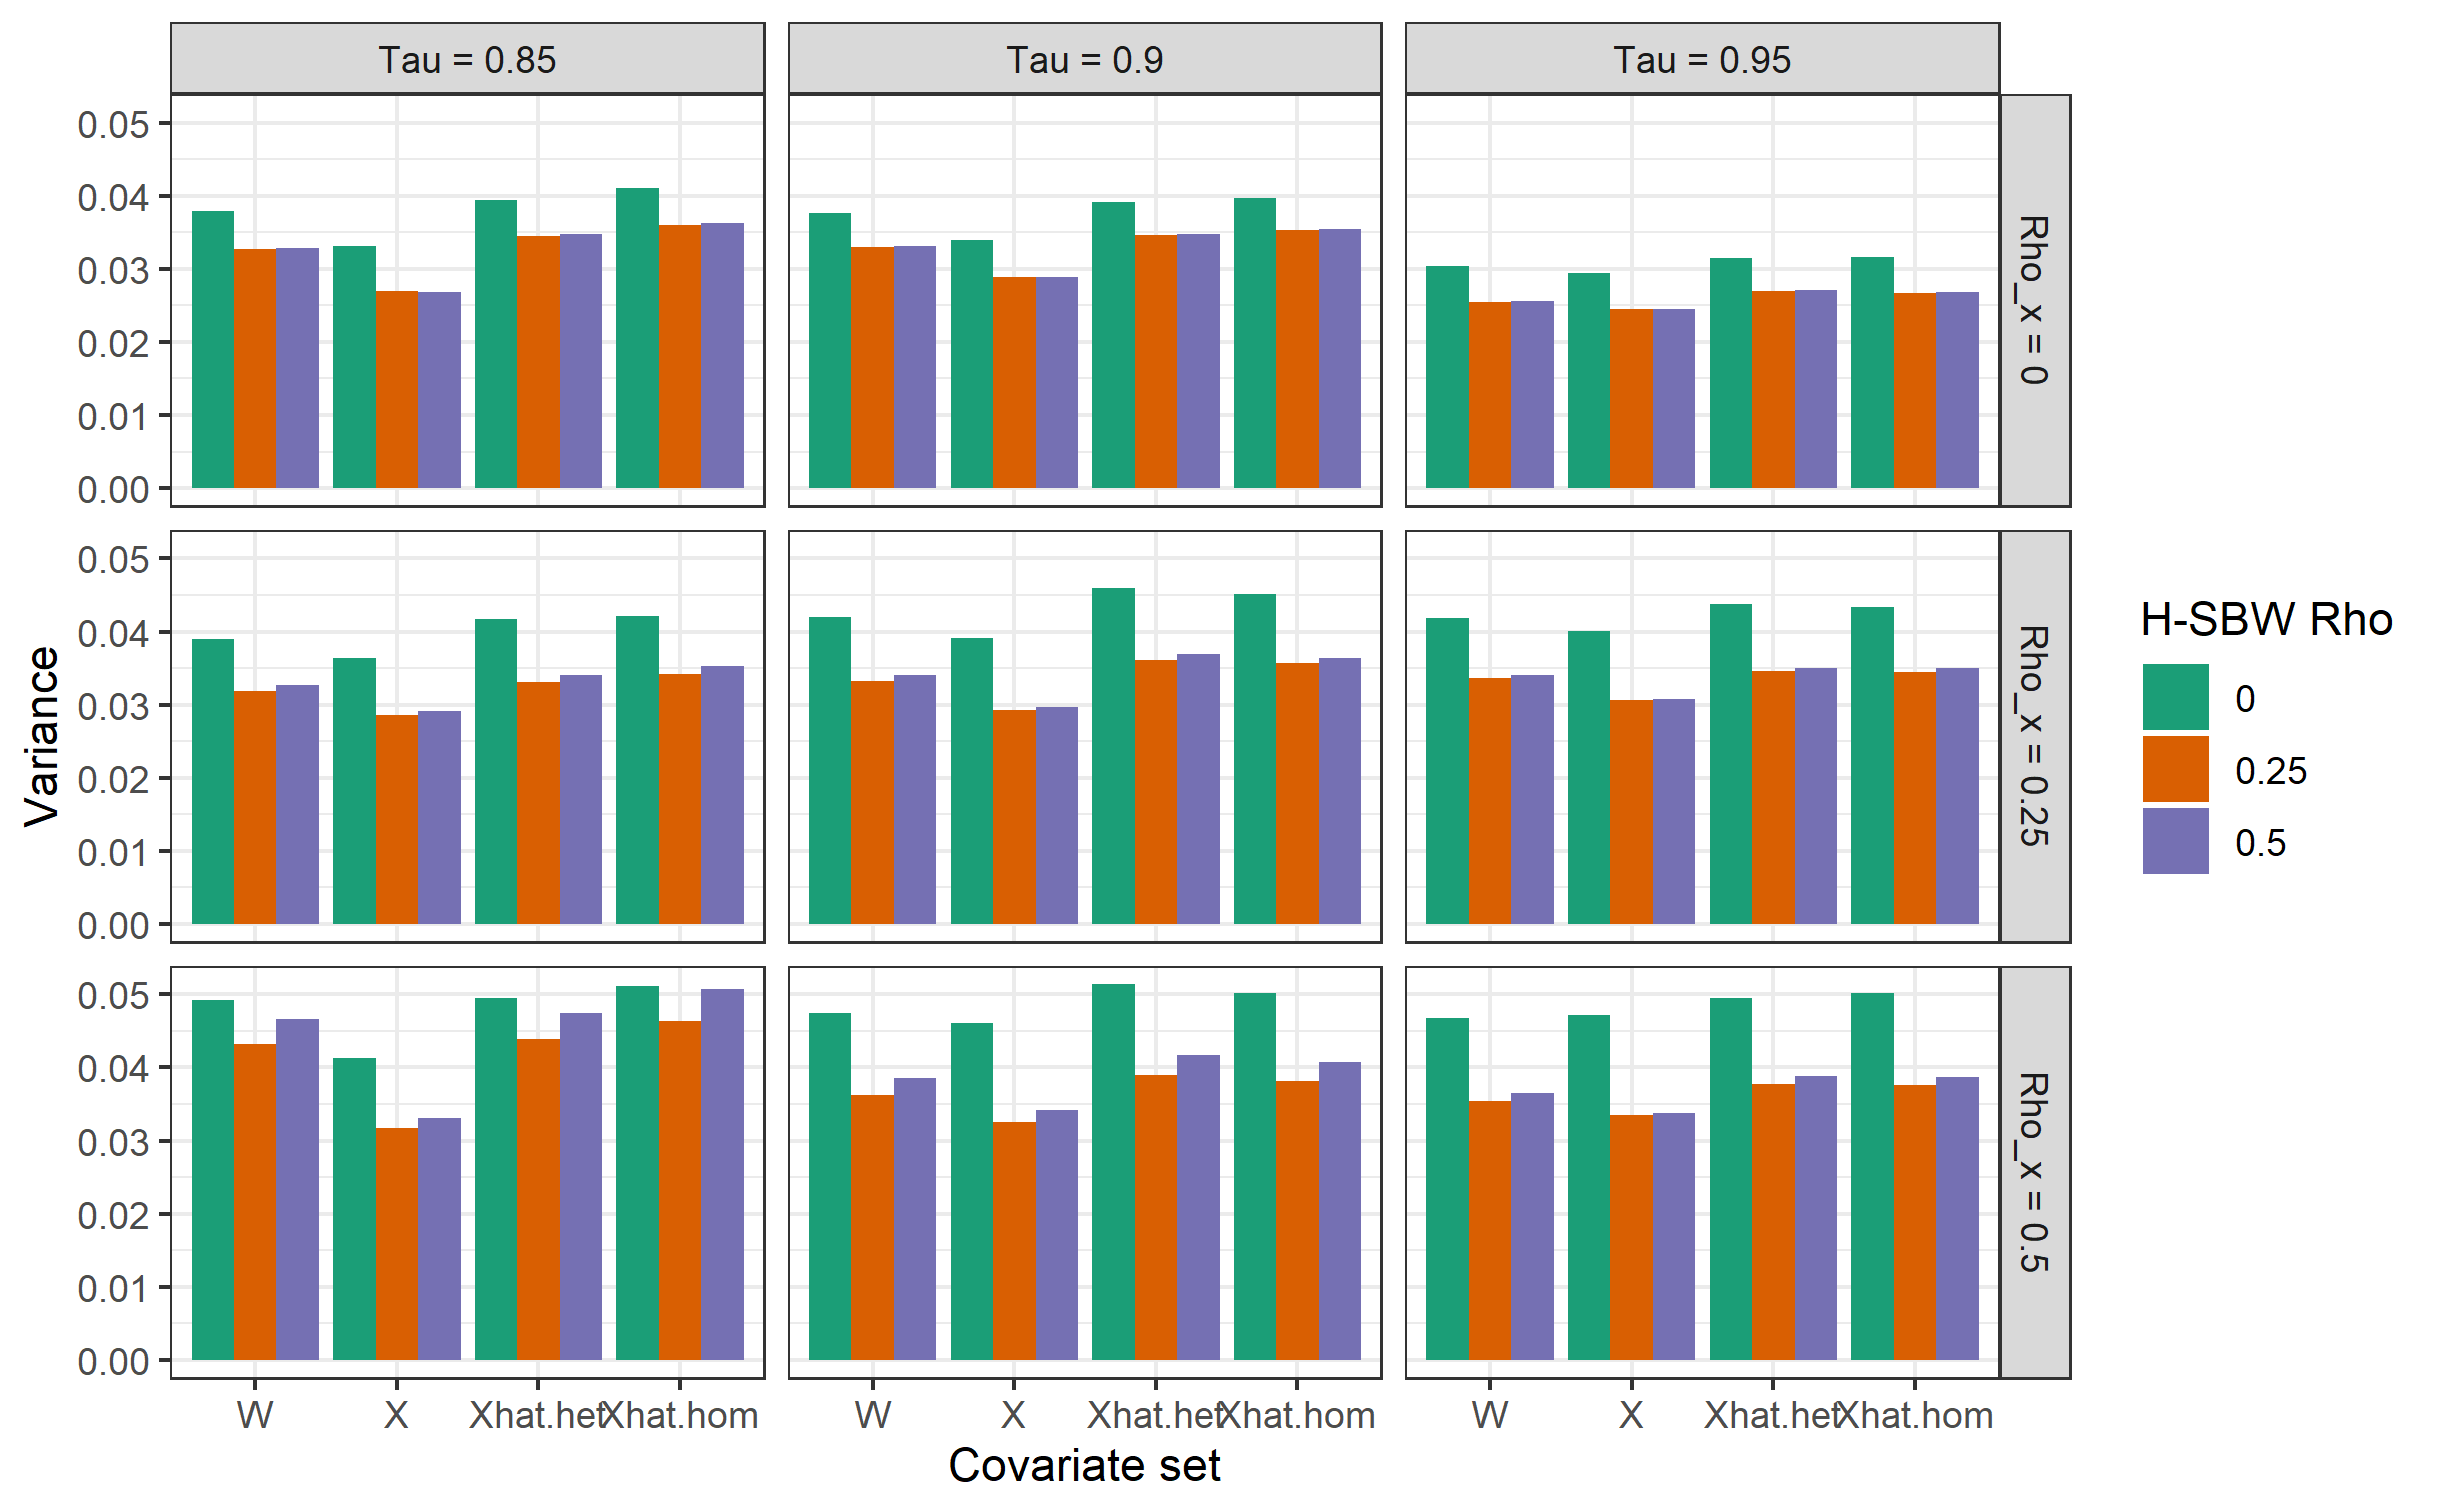
\includegraphics[scale=0.5]{01_Plots/var-plot.png}
    \subcaption{Averaged across 500 simulations for each specification}
\end{center}
\end{figure}

In Figure~\ref{fig:simmse} we display the MSE of these estimators (we remove $\tilde{X}_{A=1}^{cor}$ since we have already seen that it has poor performance relative to the other procedures considered). We find that despite the increase in bias for H-SBW with $\hat{X}_{A=1}^{hom}$ or $\hat{X}_{A=1}^{het}$, we may still find a modest MSE reduction. Of course, whether or not there are MSE reductions more generally also depends on $\rho_y$, which we have fixed here throughout: if we were to set $\rho_y = 0$, we would expect the MSE of these estimators to increase with $\rho$, even when we observe $X$. 

\begin{figure}[H]
\begin{center}
    \caption{Simulation study: estimator mean-square-error}\label{fig:simmse}
    \label{fig:loveplotc1}
    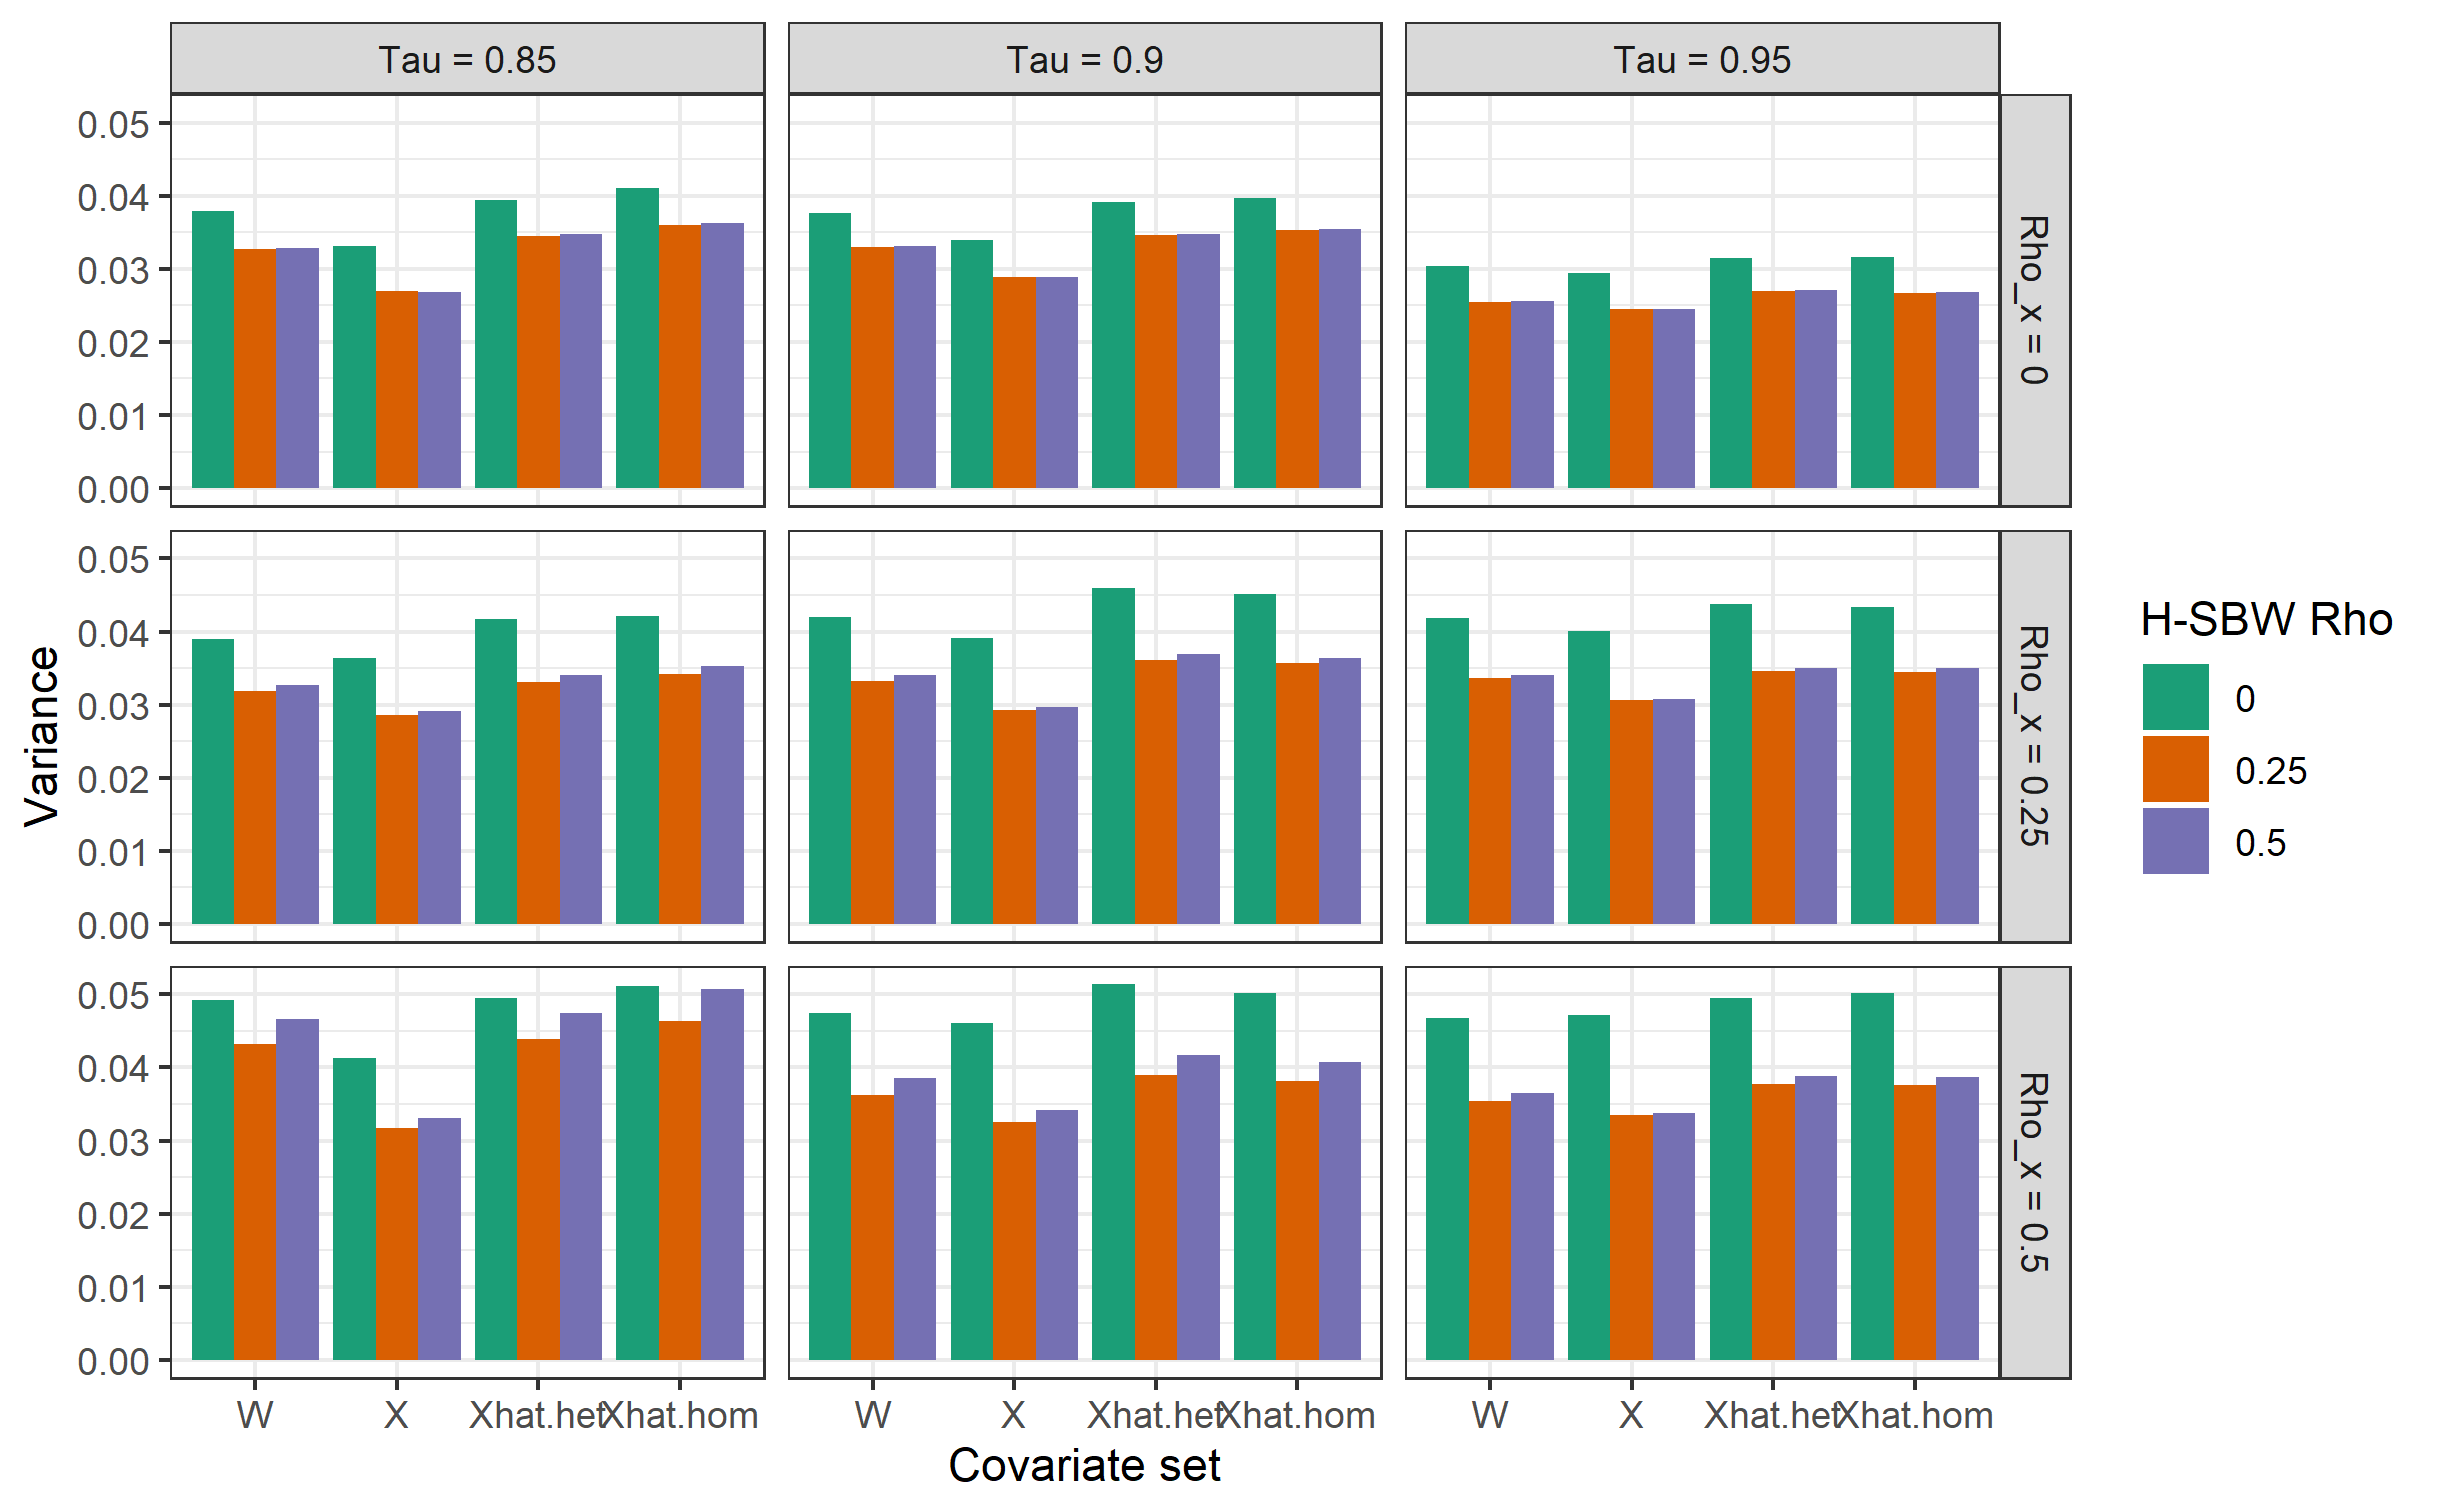
\includegraphics[scale=0.5]{01_Plots/var-plot.png}
    \subcaption{Averaged across 500 simulations for each specification}
\end{center}
\end{figure}

Finally, we evaluate the performance of the leave-one-state-out jackknife procedure and evaluate confidence interval coverage and length. We display these results in Figures~\ref{fig:simcoverage1} and ~\ref{fig:simcoverage2}. 

We first discuss Figure~\ref{fig:simcoverage1}. When $\rho = 0$ we find that we obtain approximately nominal coverage rates across all specifications that use $X$ or some version of $\hat{X}$. However, we fail to get even close to nominal coverage rates when balancing on $W$, even when $\tau$ is quite high. We do see the performance of our estimates deteriorate as we increase $\rho_x$, even when balancing on the true covariates. We also see that our coverage rates tend to get worse for $\hat{X}^{het}$ and $\hat{X}^{hom}$ in the settings where we found the highest bias. On the other hand, we also find that our coverage rates are often quite conservative, particularly for estimators generated on $\hat{X}$. 

\begin{figure}[H]
\begin{center}
    \caption{Simulation study: jackknife coverage rates}\label{fig:simcoverage1}
    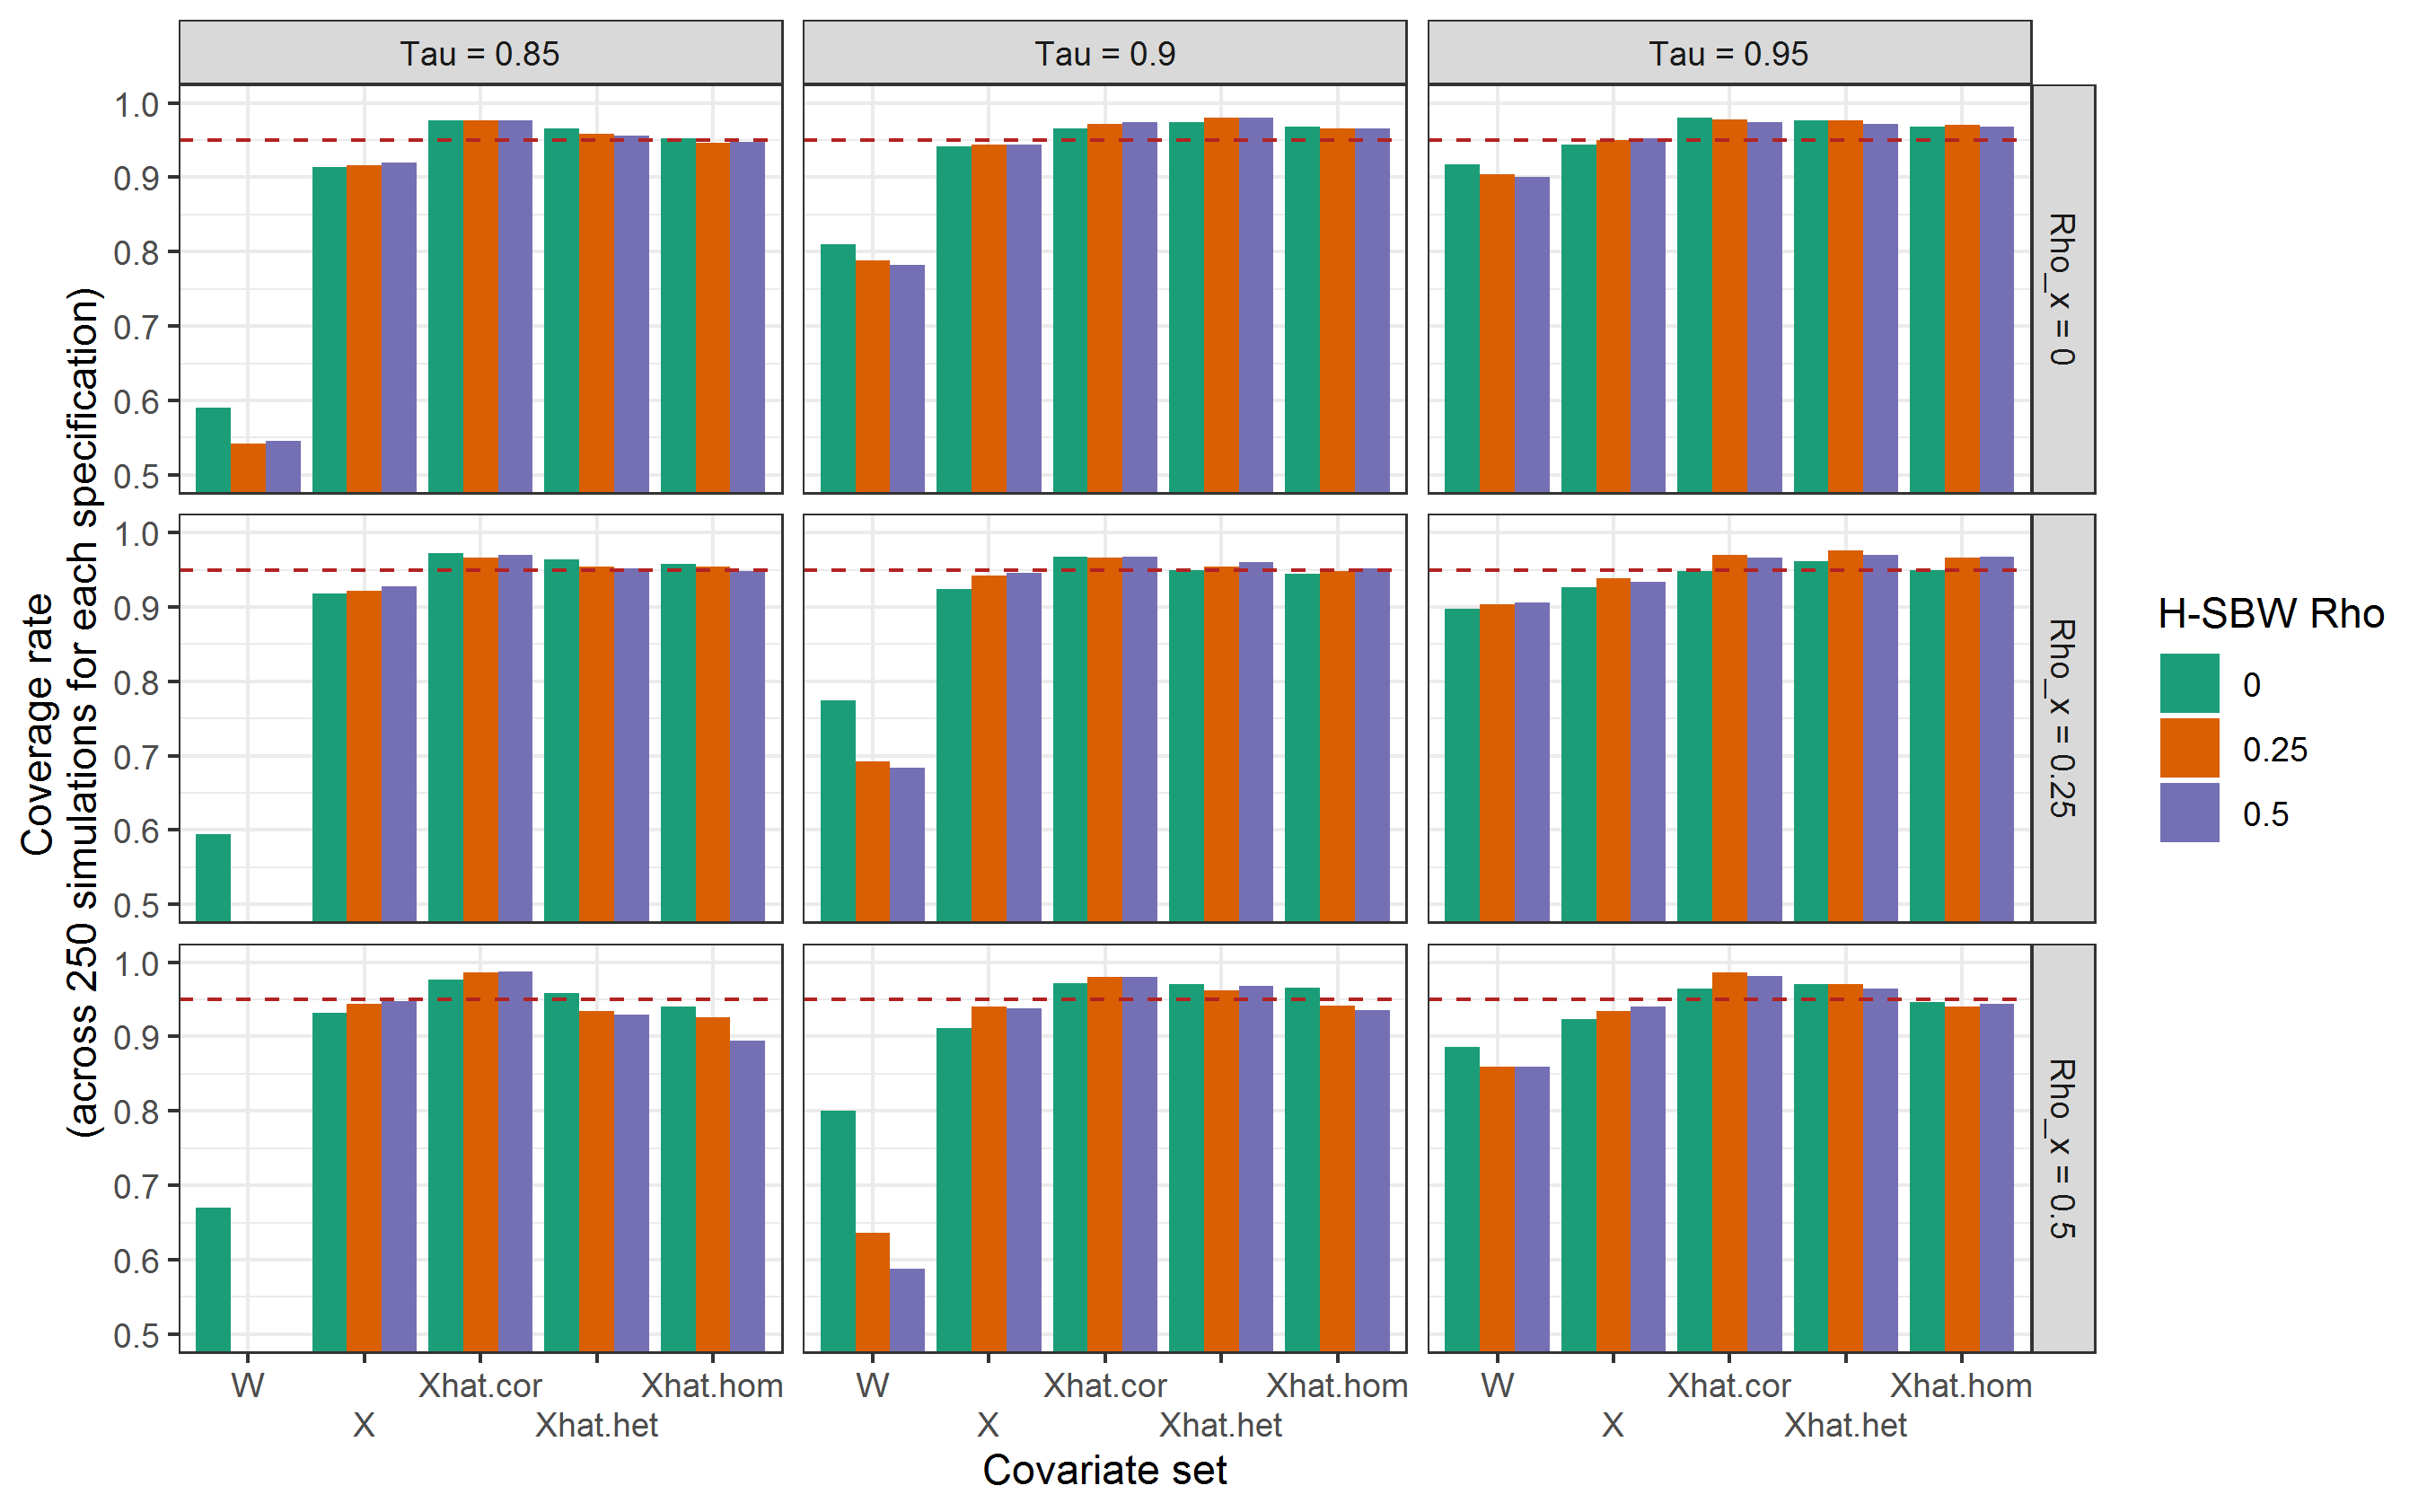
\includegraphics[scale=0.5]{01_Plots/coverage-plot-1.png}
    \subcaption{Averaged across 500 simulations for each specification}
\end{center}
\end{figure}

The figure displays one final and subtle but interesting feature: when we observe $X$, setting $\rho > 0$ appears to improve the coverage rates. We speculate this may be because H-SBW more evenly dispersing weights across states, increasing the ``effective sample size'' of the states, and thereby improving the asymptotic approximation of the variance estimates. We explore this feature more in Section~\ref{appssec:simstudyresults2} for different parameterizations of $\rho_y$. 

Finally, in Figure~\ref{fig:ciwdth} we evaluate the confidence interval lengths. As expected, we find that the H-SBW estimator is associated with lower lengths, reflecting that the estimators have decreased variability under our correlation structures. The optimal $\rho$ throughout is 0.25; however, we see that even $\rho = 0.5$ we obtain more precise inferences than when $\rho = 0$. Of course, in the context of measurement error, this also risks inducing more bias, though without measurement error this suggests benefits to using H-SBW even when our estimate of $\rho$ is a guess. All results are similar when considering homoskedastic measurement errors. 

\begin{figure}[H]\label{fig:ciwidth}
\begin{center}
    \caption{Confidence interval length}\label{fig:simcoverage2}
    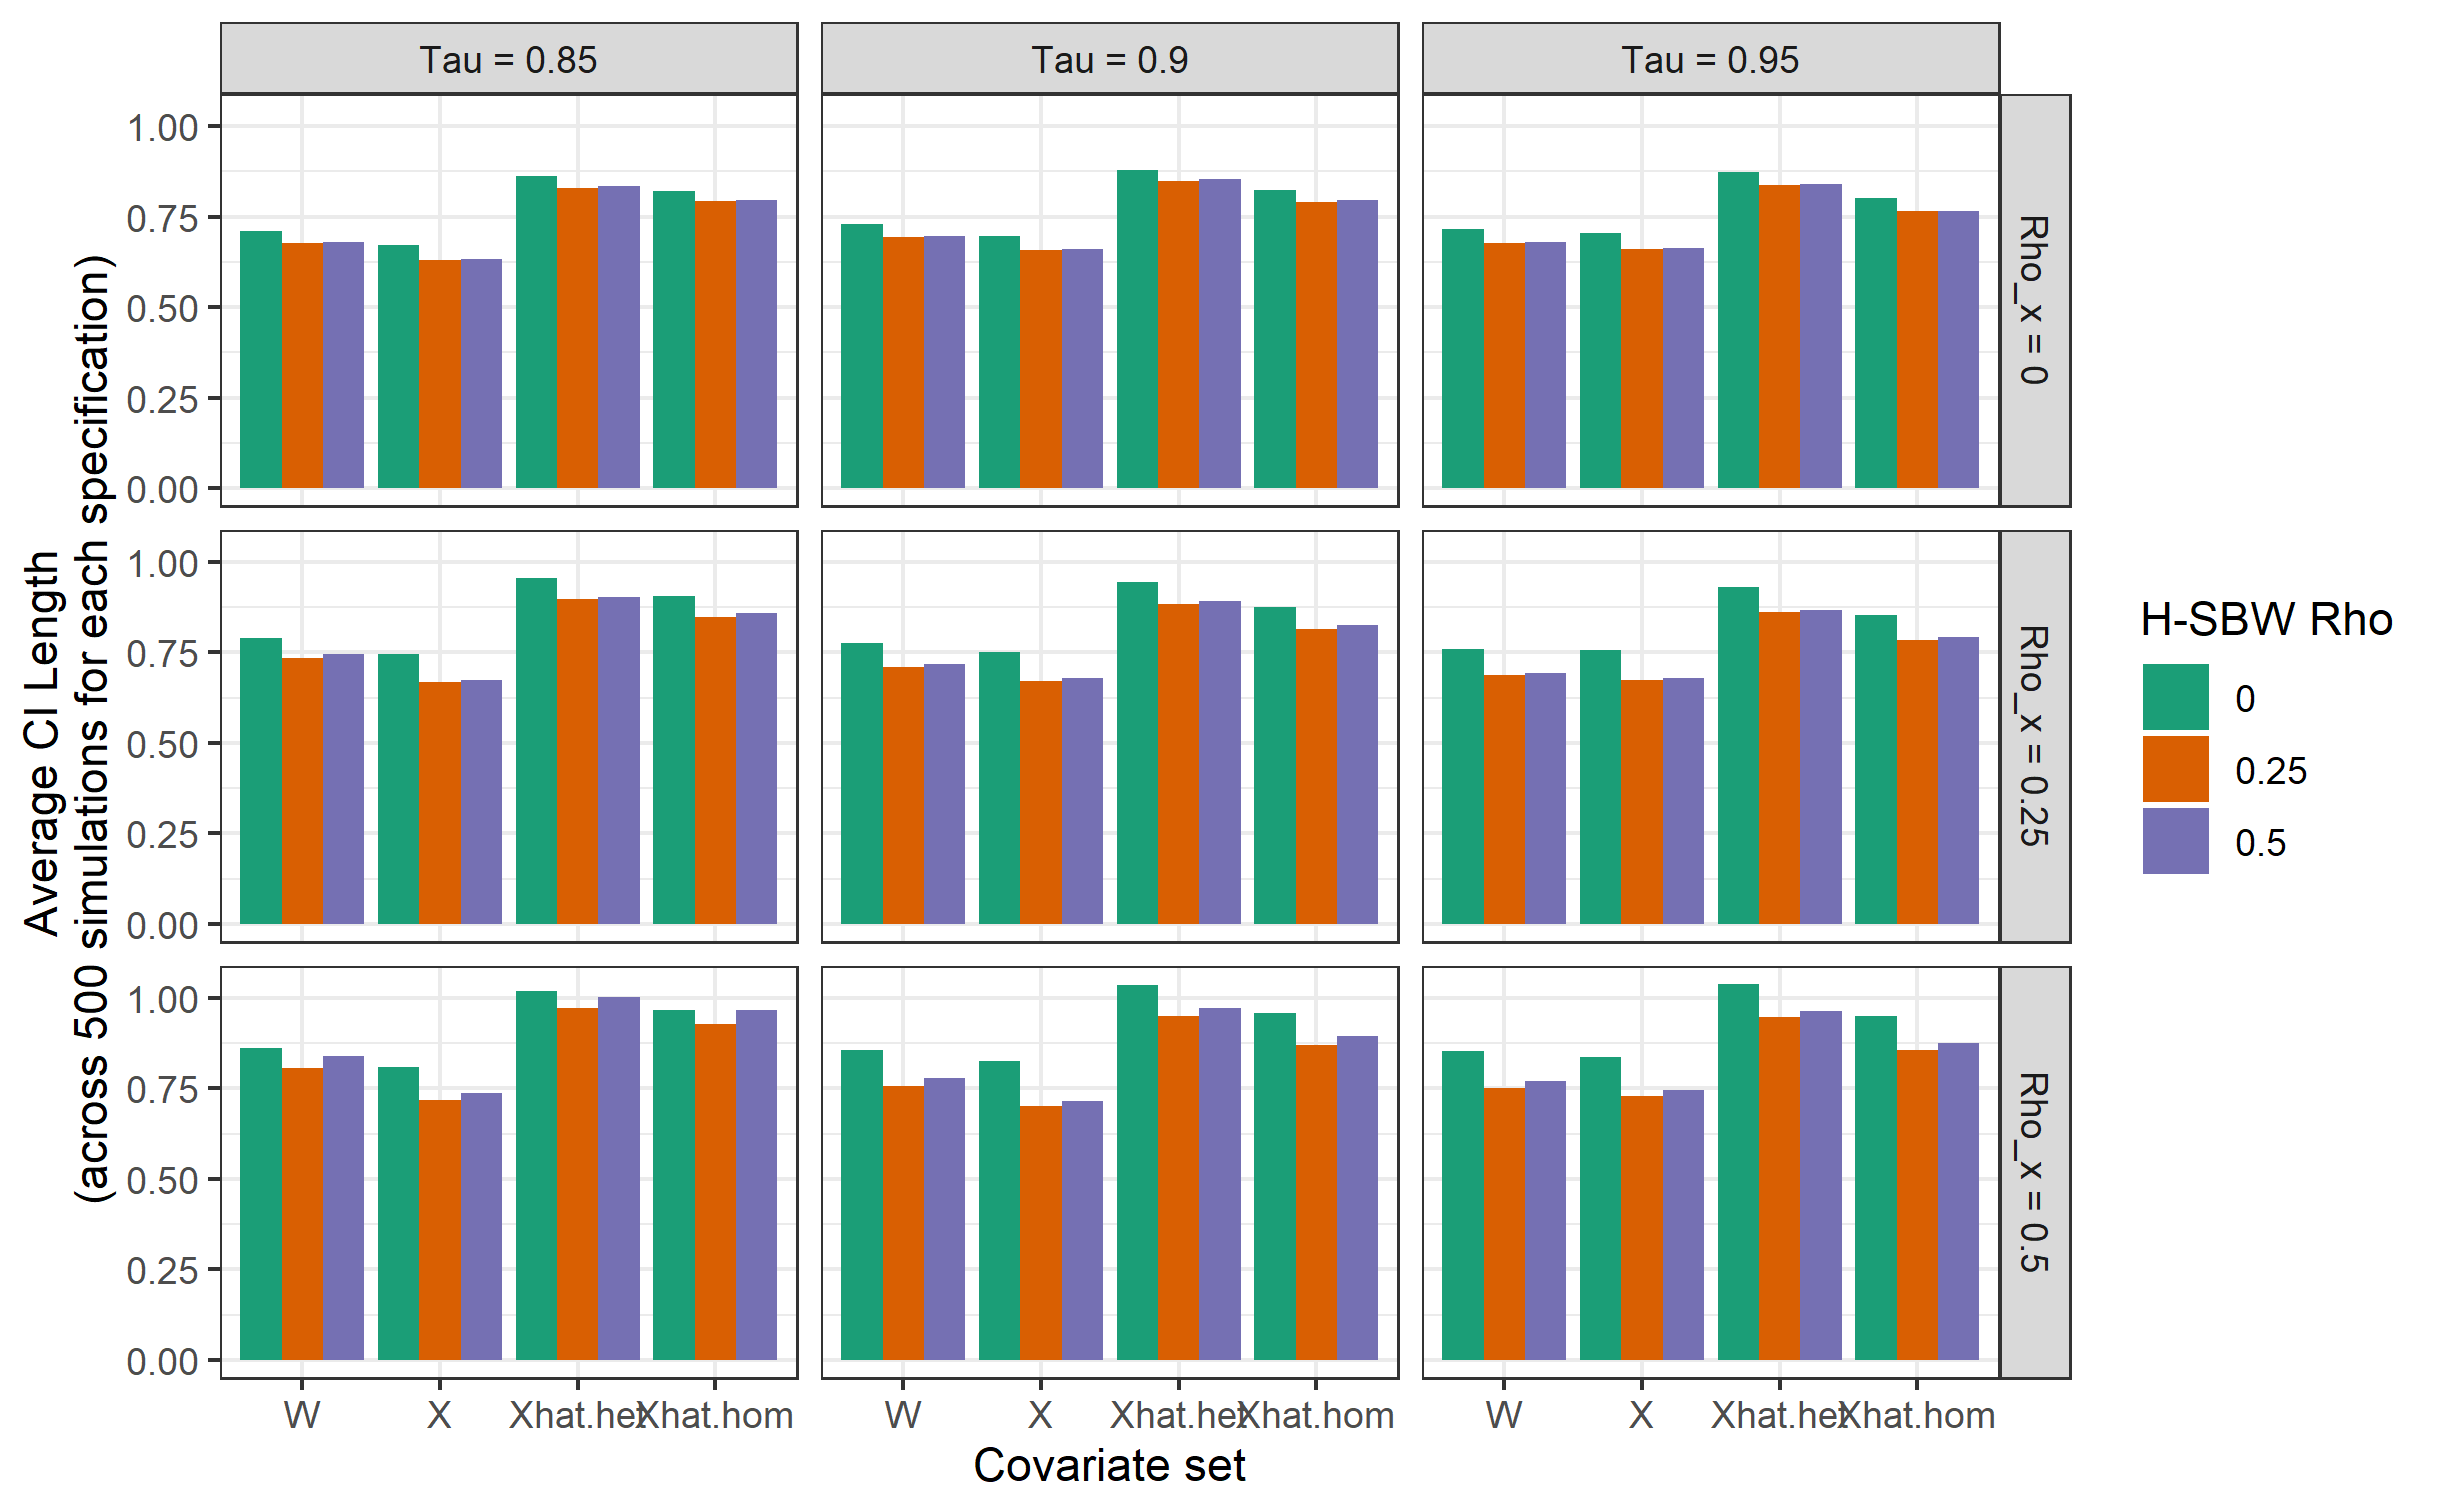
\includegraphics[scale=0.5]{01_Plots/ci-length-plot.png}
    \subcaption{Averaged across 500 simulations for each specification}
\end{center}
\end{figure}

We emphasize three takeaways from this simulation study. First, we do not find any evidence that the ``heterogeneous adjustment'' improves our estimates along any dimension, even in an ideal setting. However, this may in part reflect the distribution of sample sizes we generated, which we took to be uniform; perhaps with a different distribution these results would differ. Second, while setting $\rho > 0$ can increase the bias of our estimates in the context of measurement error, the bias is generally small relative to the bias of balancing on the noisy covariate measurements $W$. Even so, MSE improvements using H-SBW are still possible relative to SBW if we assume some non-negligible state-level random effect and relatively small measurement error. Third, accounting for the correlation in the data when using H-SBW and the data are measured with error may not be worth it given a small sample of states, despite the improved theoretic properties. This simulation study assumes throughout that we know the true data generating model for the outcome, and that are data are Gaussian. This study complements our validation study in Section~\ref{sec:results}, which has more direct bearing on understanding how these estimators might perform in our application.

\subsubsection{Additional results}\label{appssec:simstudyresults2}

In this subsection we demonstrate two additional results: first, that the correlated adjustment procedure proposed in Appendix~\ref{app:adjustmentdetails} is consistent as $m \to \infty$. Second, we consider confidence interval coverage for H-SBW with known covariates $X$, setting $m = 25$ but varying $\rho_y$, and demonstrate that H-SBW can improve the corresponding coverage rates relative to SBW when using the leave-one-state-out jackknife. 